Insert data into the \texttt{MY\_EMPLOYEE} table.
\begin{enumerate}
%%%%%%%Problem 1%%%%%%%%%%%
    \item Run the statement in the \texttt{lab8\_1.sql} script to build the \texttt{MY\_EMPLOYEE} table to be used for the lab.
    
    \textbf{Solution: }
    \begin{lstlisting}[language=SQL]
create table my_employee(
    id number (4) 
        constraint my_employee_id_not_null not null,
    last_name varchar2(25),
    first_name varchar2(25),
    userId varchar2(8),
    salary number (9,2)
);
    \end{lstlisting}
%%%%%%%Problem 2%%%%%%%%%%%
    \item Describe the structure of the \texttt{MY\_EMPLOYEE} table to identify the column names. 
    \begin{figure}[h]
        \centering
        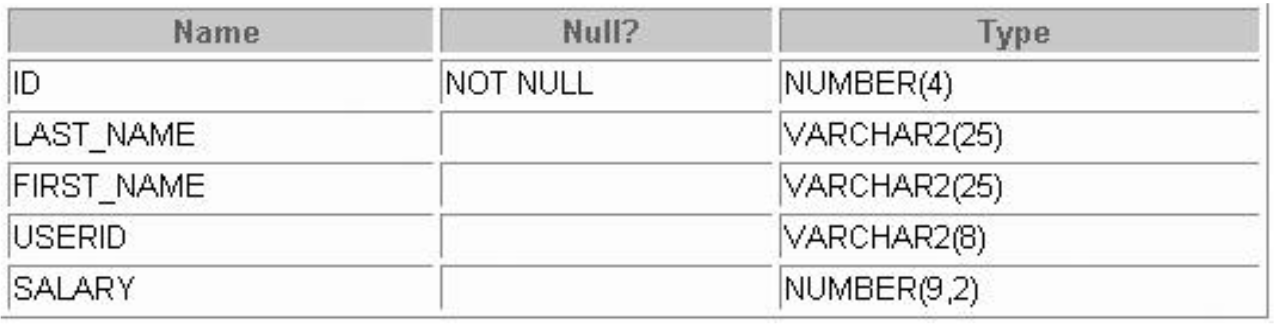
\includegraphics[width=0.7\linewidth]{graphics/82.png}
    \end{figure}
    
    \textbf{Solution: }
    \begin{lstlisting}[language=SQL]
describe my_employee;
    \end{lstlisting}
%%%%%%%Problem 3%%%%%%%%%%%
    \item  Add the first row of data to the \texttt{MY\_EMPLOYEE} table from the following sample data. Do not list the
columns in the INSERT clause.   
    \begin{figure}[h]
        \centering
        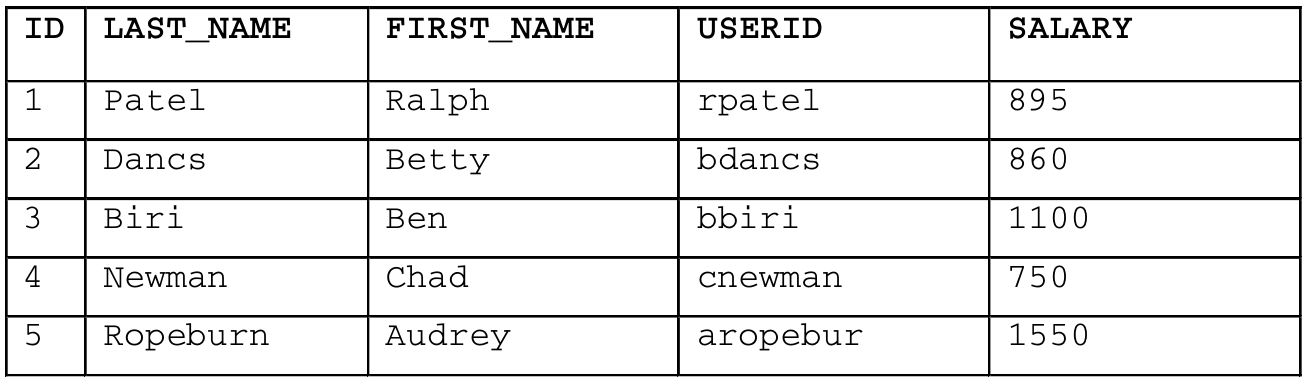
\includegraphics[width=0.7\linewidth]{graphics/83.png}
    \end{figure}

    \textbf{Solution: }
    \begin{lstlisting}[language=SQL]
insert into my_employee
values (1, 'Patel', 'Ralph', 'rpatel', 895);
    \end{lstlisting}
%%%%%%%Problem 4%%%%%%%%%%%
    \item  Populate the \texttt{MY\_EMPLOYEE} table with the second row of sample data from the preceding list. This
time, list the columns explicitly in the INSERT clause.  
    
    \textbf{Solution: }
    \begin{lstlisting}[language=SQL]
insert into my_employee(id,last_name,first_name,userId,salary)
values (2,'Dancs','Betty','bdancs',860);  
    \end{lstlisting}
%%%%%%%Problem 5%%%%%%%%%%%
    \item  Confirm your addition to the table.   
    
    \textbf{Solution: }
    \begin{lstlisting}[language=SQL]
select * 
from my_employee;
    \end{lstlisting}
\begin{figure}[h]
    \centering
    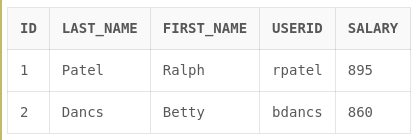
\includegraphics[width=0.7\linewidth]{graphics/p85.png}
\end{figure}
%%%%%%%Problem 6%%%%%%%%%%%
    \item  Write an INSERT statement in a text file named loademp.sql to load rows into the
\texttt{MY\_EMPLOYEE} table. Concatenate the first letter of the first name and the first seven characters of
the last name to produce the user ID.  
    
    \textbf{Solution: }skipped(sql*plus required).
    \begin{lstlisting}[language=SQL]
    \end{lstlisting}
%%%%%%%Problem 7%%%%%%%%%%%
    \item  Populate the table with the next two rows of sample data by running the INSERT statement in the
script that you created. 
    
    \textbf{Solution: }skipped(sql*plus required).
    \begin{lstlisting}[language=SQL]
    \end{lstlisting}
%%%%%%%Problem 8%%%%%%%%%%%
    \item  Confirm your additions to the table.
    \begin{figure}[h]
        \centering
        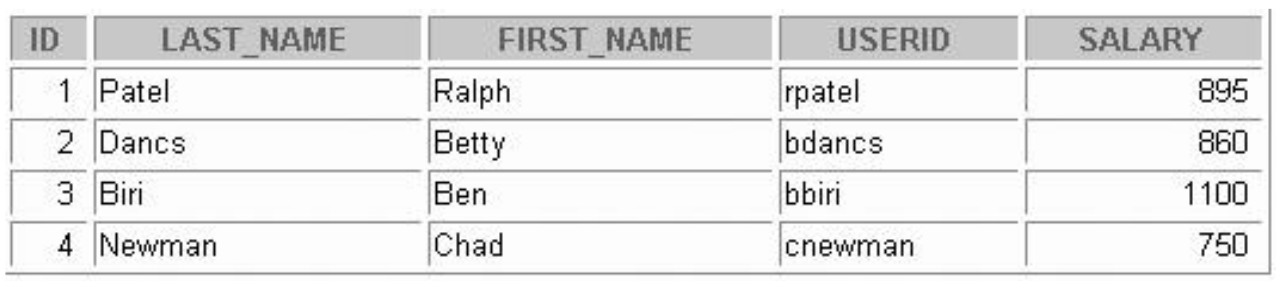
\includegraphics[width=0.9\linewidth]{graphics/88.png}
    \end{figure}
    \textbf{Solution: }
    \begin{lstlisting}[language=SQL]
select *
from my_employee;
    \end{lstlisting}
%%%%%%%Problem 9%%%%%%%%%%%
    \item  Make the data additions permanent.
    
    \textbf{Solution: }
    \begin{lstlisting}[language=SQL]
Commit;
    \end{lstlisting}

Update and delete data in the \texttt{MY\_EMPLOYEE} table.
%%%%%%%Problem 10%%%%%%%%%%%
    \item  Change the last name of employee 3 to Drexler.
    
    \textbf{Solution: }
    \begin{lstlisting}[language=SQL]
-- adding the remaining rows to move forward
insert into my_employee
values (3, 'Biri', 'Ben', 'bbiri', 1100);
insert into my_employee
values (4, 'Newman', 'Chad', 'cnewman', 750);
insert into my_employee
values (5, 'Ropeburn', 'Audrey', 'aropebur', 1550);
    \end{lstlisting}
    \begin{lstlisting}[language=SQL]
update my_employee
set last_name = 'Drexler'
where id = 3;
    \end{lstlisting}
%%%%%%%Problem 11%%%%%%%%%%%
    \item  Change the salary to 1000 for all employees with a salary less than 900.
    
    \textbf{Solution: }
    \begin{lstlisting}[language=SQL]
update my_employee
set salary = 1000
where salary < 900;
    \end{lstlisting}
%%%%%%%Problem 12%%%%%%%%%%%
    \item  Verify your changes to the table.
    
    \textbf{Solution: }
    \begin{lstlisting}[language=SQL]
select id,last_name, salary
from my_employee;
    \end{lstlisting}
    
    \textbf{Output: }
    \begin{figure}[h]
        \centering
        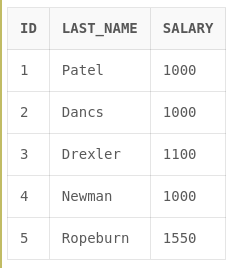
\includegraphics[width=0.4\linewidth]{graphics/p812.png}
    \end{figure}
%%%%%%%Problem 13%%%%%%%%%%%
    \item  Delete Betty Dancs from the \texttt{MY\_EMPLOYEE} table.
    
    \textbf{Solution: }
    \begin{lstlisting}[language=SQL]
delete
from my_employee
where last_name = 'Dancs' and first_name = 'Betty';
    \end{lstlisting} 
%%%%%%%Problem 14%%%%%%%%%%%
    \item  Confirm your changes to the table.
    
    \textbf{Solution: }
    \begin{lstlisting}[language=SQL]
select * 
from my_employee 
where last_name = 'Dancs' and first_name = 'Betty';

--No data found --
    \end{lstlisting} 
%%%%%%%Problem 15%%%%%%%%%%%
    \item  Commit all pending changes.
    
    \textbf{Solution: }
    \begin{lstlisting}[language=SQL]
Commit;
    \end{lstlisting}  
Control data transaction to the \texttt{MY\_EMPLOYEE} table.
%%%%%%%Problem 16%%%%%%%%%%%
    \item Populate the table with the last row of sample data by modifying the statements in the script that you
created in step 6. Run the statements in the script.
    
    \textbf{Solution: }skipped(sql*plus required)
    \begin{lstlisting}[language=SQL]
    \end{lstlisting}  
%%%%%%%Problem 17%%%%%%%%%%%
    \item Confirm your addition to the table.
    
    \textbf{Solution: }skipped
    \begin{lstlisting}[language=SQL]
    \end{lstlisting} 
%%%%%%%Problem 18%%%%%%%%%%%
    \item Mark an intermediate point in the processing of the transaction.
    
    \textbf{Solution: }
    \begin{lstlisting}[language=SQL]
SAVEPOINT before_deletion;
    \end{lstlisting}
%%%%%%%Problem 19%%%%%%%%%%%
    \item Empty the entire table.
    
    \textbf{Solution: }
    \begin{lstlisting}[language=SQL]
delete from my_employee;
    \end{lstlisting}
%%%%%%%Problem 20%%%%%%%%%%%
    \item Confirm that the table is empty.
    
    \textbf{Solution: }
    \begin{lstlisting}[language=SQL]
select *
from my_employee;
    \end{lstlisting}
%%%%%%%Problem 21%%%%%%%%%%%
    \item Discard the most recent DELETE operation without discarding the earlier INSERT operation.
    
    \textbf{Solution: }
    \begin{lstlisting}[language=SQL]
ROLLBACK TO before_deletion;
    \end{lstlisting}
%%%%%%%Problem 22%%%%%%%%%%%
    \newpage
    \item Confirm that the new row is still intact.
    \begin{figure}[h]
        \centering
        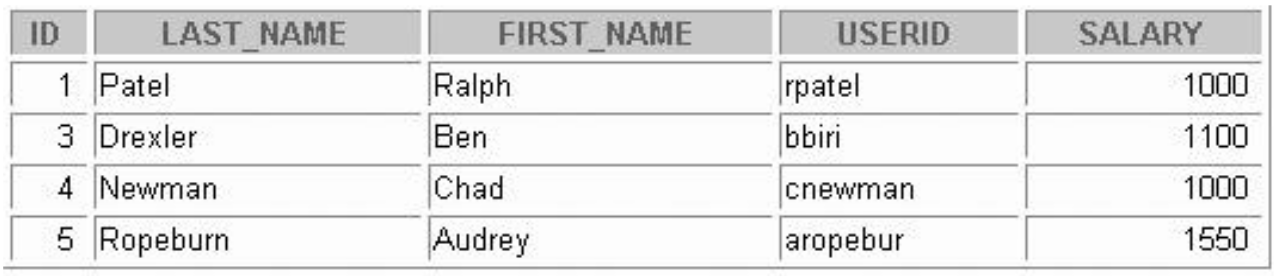
\includegraphics[width=0.9\linewidth]{graphics/822.png}
    \end{figure}

    \textbf{Solution: }
    \begin{lstlisting}[language=SQL]
select *
from my_employee;
    \end{lstlisting}
%%%%%%%Problem 23%%%%%%%%%%%
    \item Make the data addition permanent.
    
    \textbf{Solution: }
    \begin{lstlisting}[language=SQL]
Commit;
    \end{lstlisting}
\end{enumerate}